\chapter[Maxent]{Maximum Entropy}

\begin{objetivos}
By the end of this chapter, readers should understand Maxent and the maximum
entropy principle; distinguish linear, quadratic, product, hinge, and threshold
features; explain regularization; fit Maxent to \textit{Dinizia excelsa}
presence--background data; tune feature classes and the regularization
multiplier; evaluate performance independently; generate response curves and a
current suitability map; and compare Maxent with GLM, GAM, Random Forest, and BRT.
\end{objetivos}

\section{Introduction}

Maxent is among the most widely used SDM methods, especially when available data
consist of presences and background. It estimates a maximum-entropy
distribution---the most uniform distribution possible subject to constraints
imposed by environmental conditions at presence sites
\parencite{phillips2006maximum,phillips2008modeling,elith2011statistical,merow2013practical,guisan2017habitat}.

In practice, Maxent contrasts environmental values at presences with those
available in the background. It estimates a relative-suitability function that
identifies combinations resembling conditions where the species was observed.

\begin{conceito}[title={\faBook\quad Maxent in SDM}]
Maxent is a presence--background method based on maximum entropy. It estimates
a spatial distribution satisfying environmental constraints observed at
presences without assuming more structure than the available information supports.
\end{conceito}

\section{Maximum Entropy and Environmental Suitability}

Maximum entropy seeks the least biased distribution consistent with specified
constraints. In SDM, constraints derive from environmental variables at
presence locations.

\begin{equationbox}
\[
\hat{p}(x)=\frac{\exp\left(\sum_j\lambda_j f_j(x)\right)}{Z}.
\]
\end{equationbox}

Here, $\hat p(x)$ is relative suitability at location $x$, $f_j(x)$ are
functions of environmental predictors, $\lambda_j$ are estimated weights, and
$Z$ is a normalizing constant.

\section{Feature Classes}

Maxent represents species--environment relationships through feature classes:
\begin{itemize}
  \item linear (L): linear responses;
  \item quadratic (Q): unimodal or parabolic responses;
  \item product (P): interactions among predictors;
  \item hinge (H): piecewise responses and thresholds; and
  \item threshold (T): responses based on discrete cutoffs.
\end{itemize}

\begin{atencao}[title={\faExclamationTriangle\quad Maxent complexity}]
Many features combined with weak regularization can overfit. Feature classes and
regularization must therefore be tuned and evaluated outside calibration data.
\end{atencao}

\section{Regularization}

Regularization controls model complexity. Low values allow flexible responses
but increase overfitting risk. High values yield simpler, smoother models but
may fail to capture genuine ecological structure. The main tuning parameter is
the \textit{regularization multiplier}.

\begin{conceito}[title={\faBook\quad Regularization}]
Regularization penalizes excessive complexity. It is essential for spatial and
temporal transferability, particularly in future or paleoclimatic projections.
\end{conceito}

\section{Data Preparation}

The model uses the Chapter 5 presence--background dataset and Chapter 4
predictors. It is fitted with \texttt{maxnet}, an R implementation of penalized
Maxent that does not require \texttt{maxent.jar}.

\rscriptfile{scripts/unidade10/01_estrutura_pastas.R}
\rscriptfile{scripts/unidade10/02_preparar_dados_maxent.R}

\section{Tuning Feature Classes and Regularization}

Tuning compares feature-class combinations and regularization multipliers to
select a model with useful predictive performance but without unnecessary
complexity. Selection must be based on a prespecified criterion and data not
used to optimize the fitted coefficients.

\rscriptfile{scripts/unidade10/03_tuning_maxent_dinizia.R}

\begin{figure}[H]
  \centering
  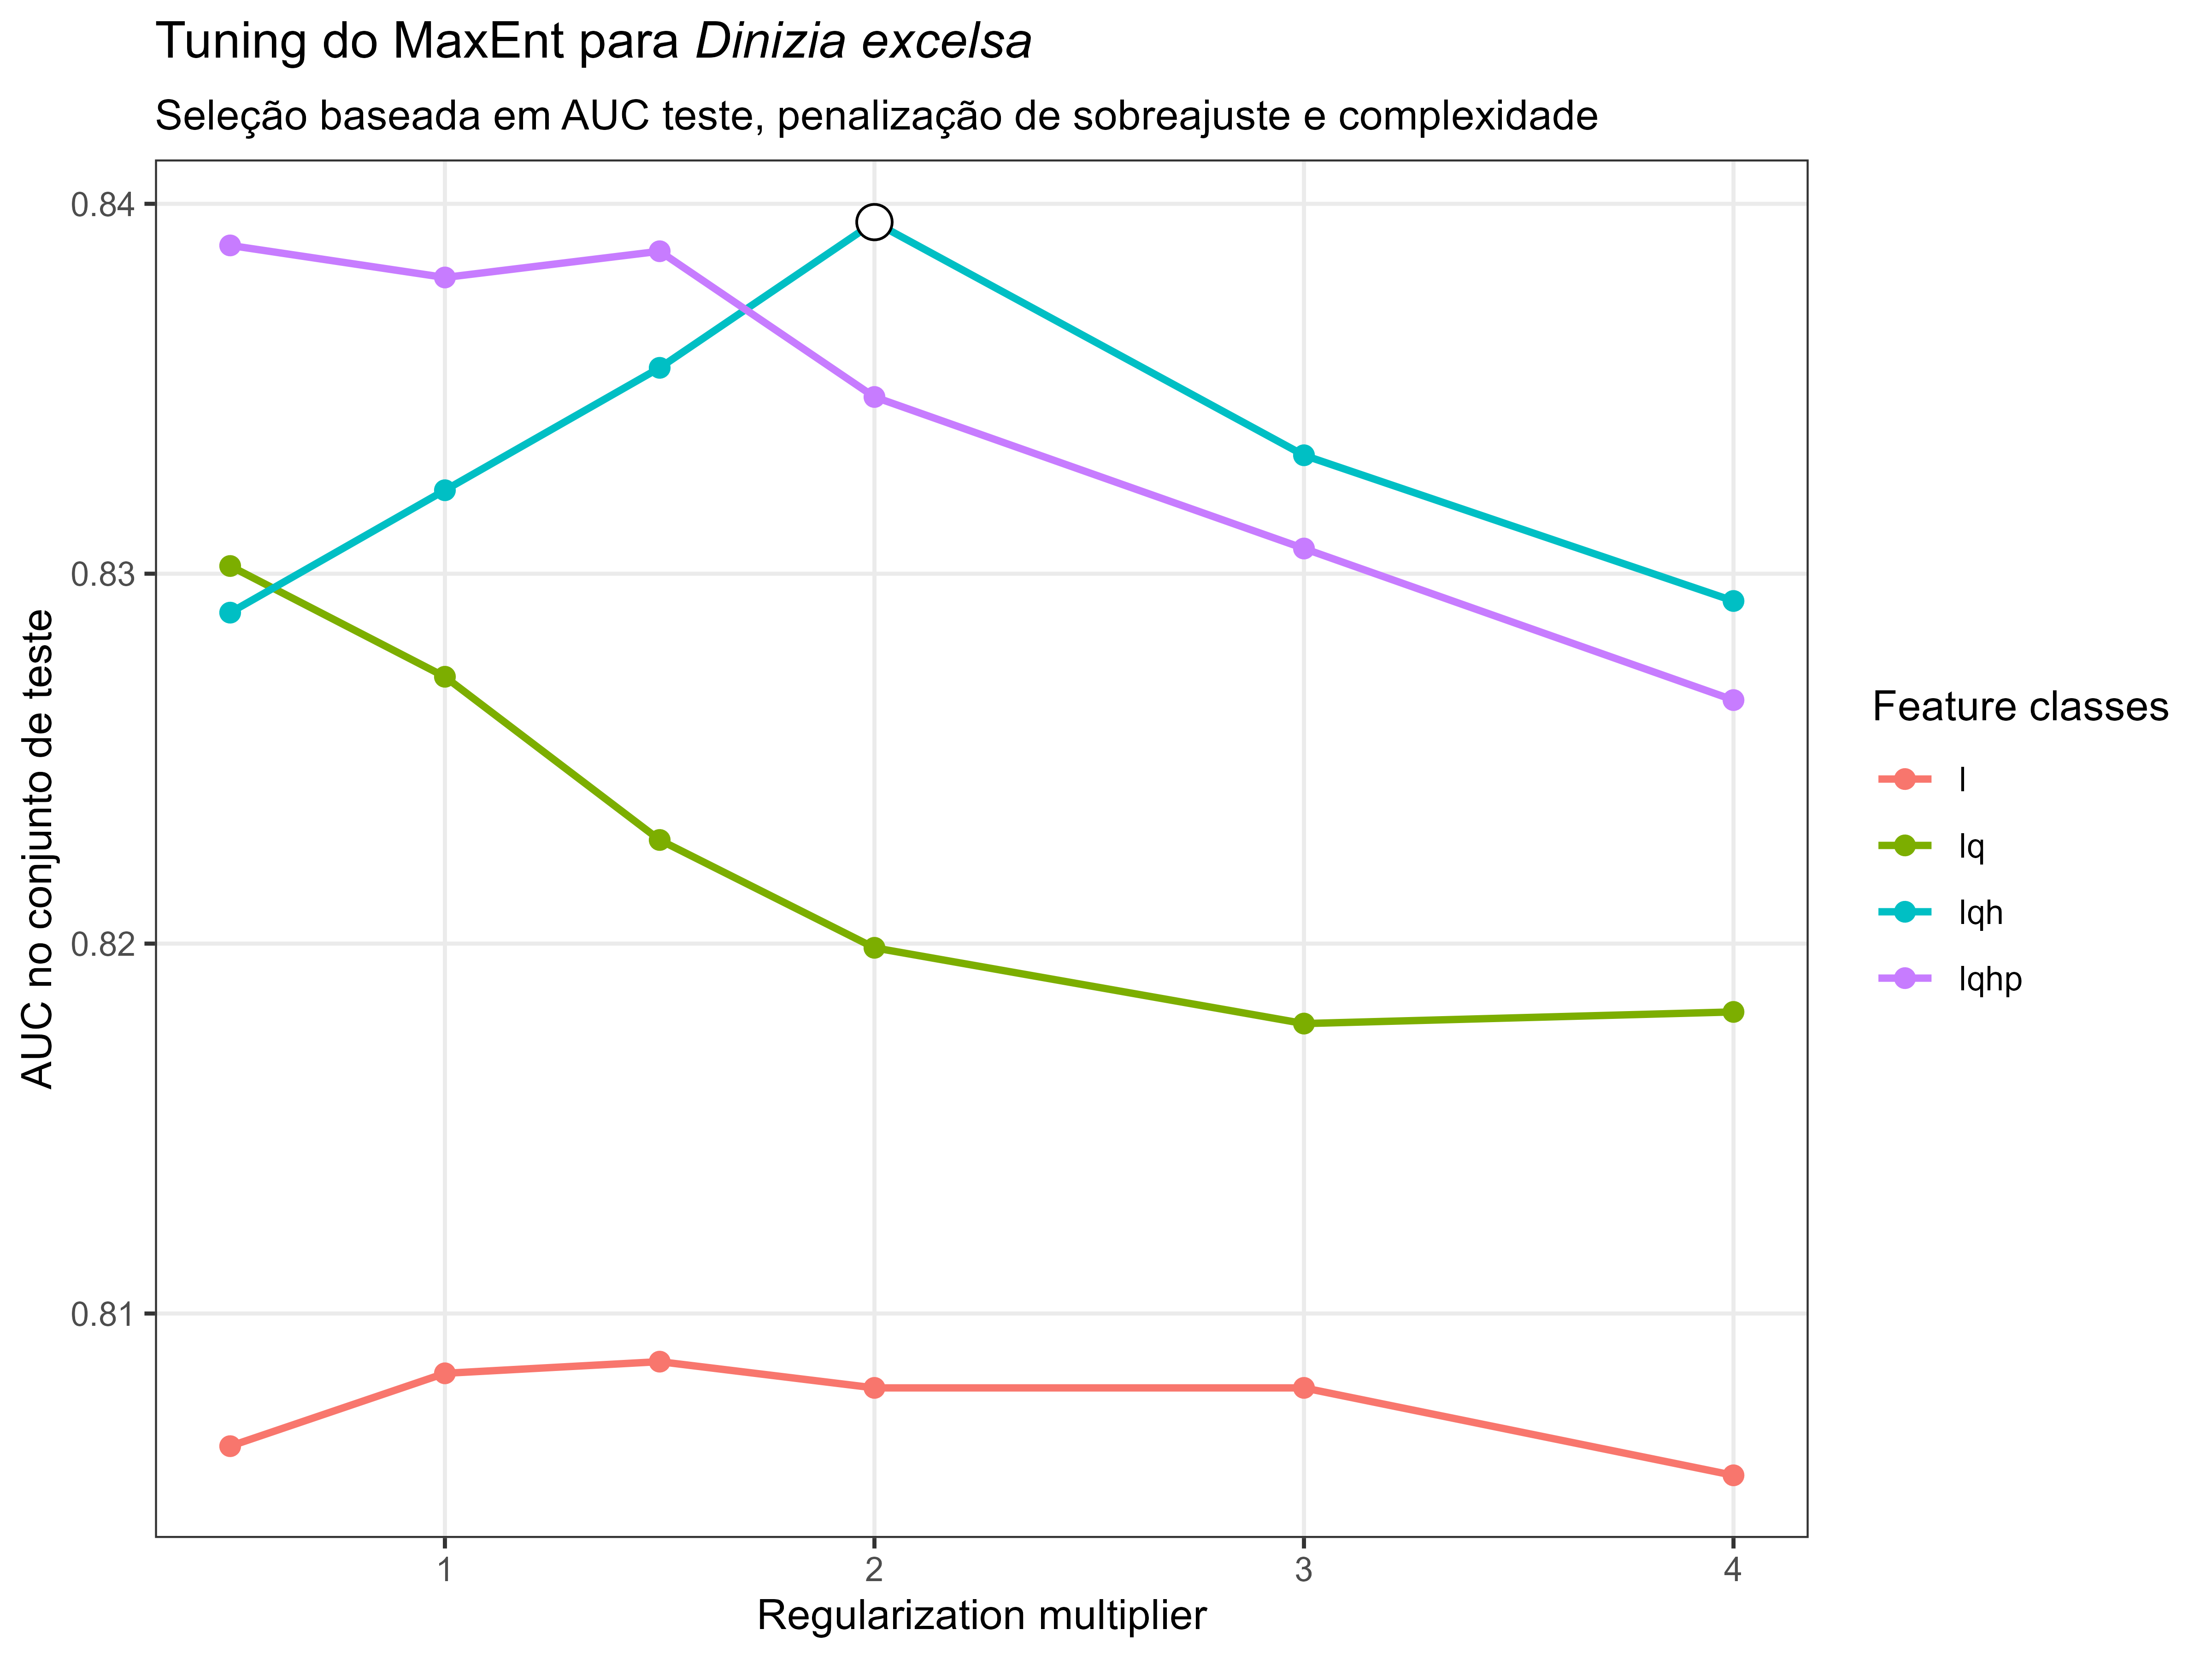
\includegraphics[width=0.88\textwidth]{figuras/unidade10/unidade10_tuning_maxent.png}
  \caption{Maxent tuning results for \textit{Dinizia excelsa} across feature-class combinations and regularization multipliers.}
  \label{fig:unidade10_tuning_maxent}
\end{figure}

\section{Fitting the Final Maxent Model}

The best supported hyperparameter combination is used to fit the final model.

\rscriptfile{scripts/unidade10/04_ajustar_maxent_final.R}

\begin{figure}[H]
  \centering
  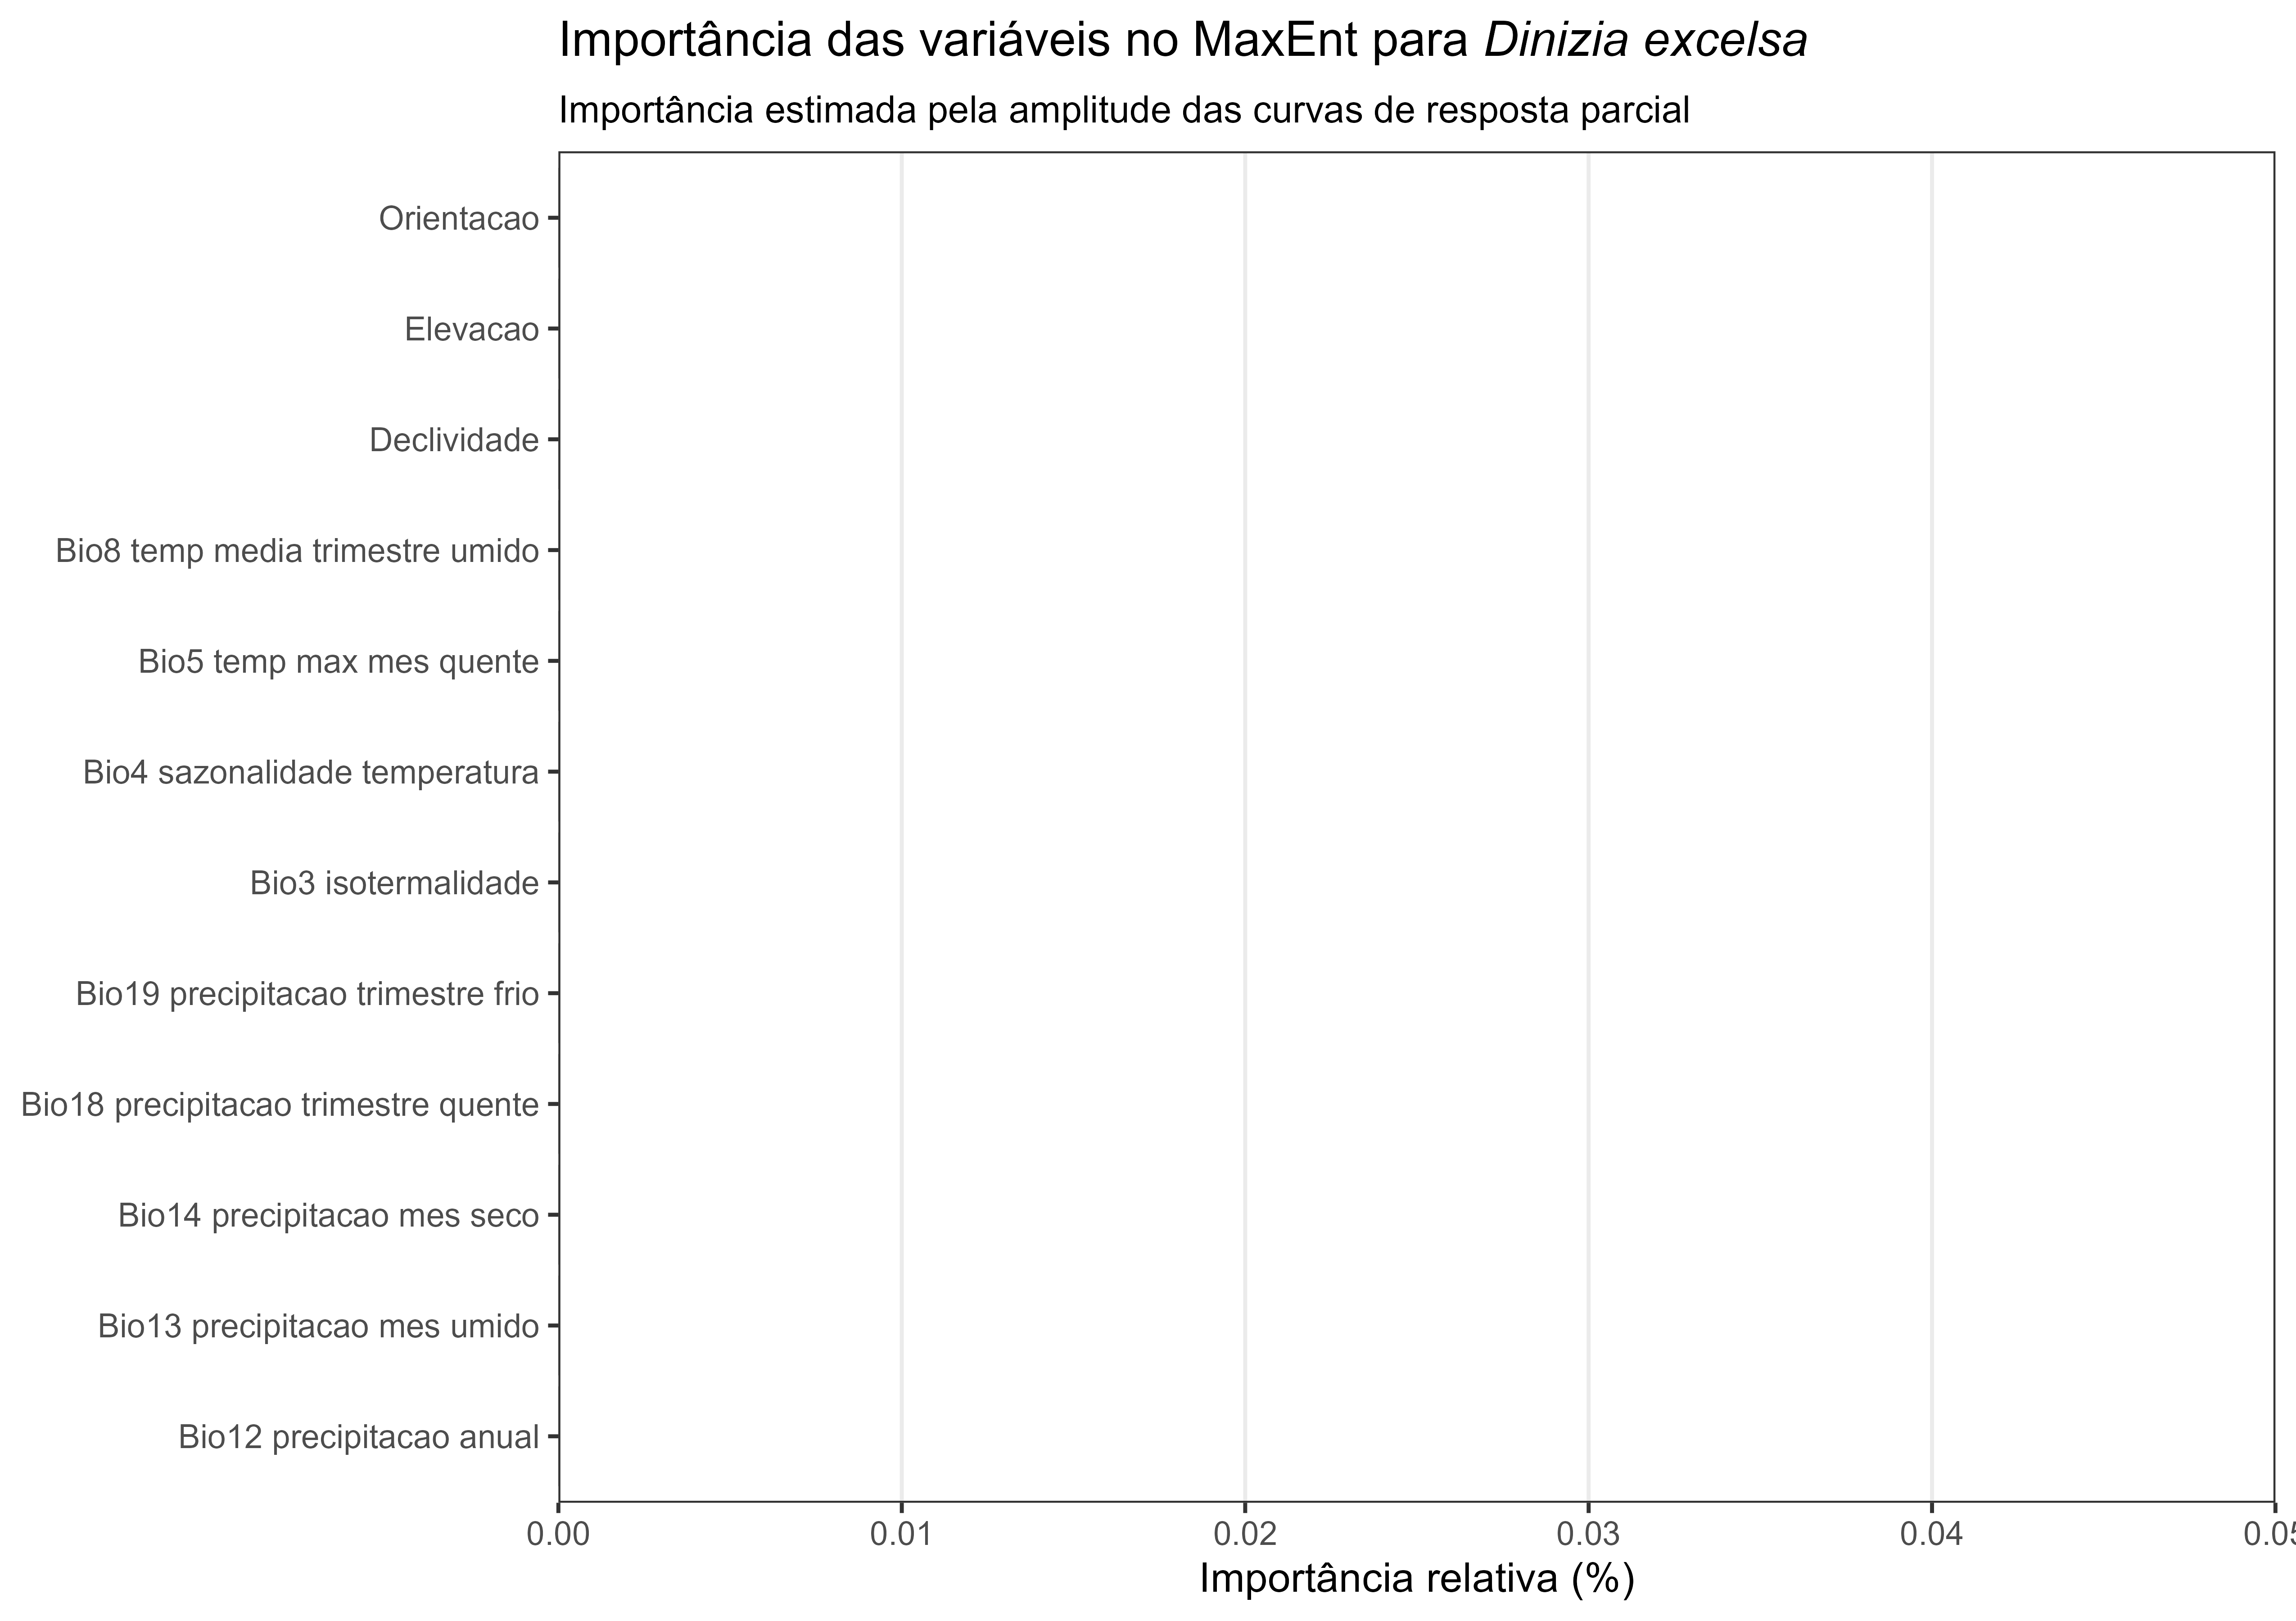
\includegraphics[width=0.86\textwidth]{figuras/unidade10/unidade10_importancia_variaveis_maxent.png}
  \caption{Relative environmental-predictor importance in the final Maxent model for \textit{Dinizia excelsa}.}
  \label{fig:unidade10_importancia_maxent}
\end{figure}

\section{Model Evaluation}

The final model is evaluated on independent test data using AUC, TSS,
sensitivity, specificity, and a confusion matrix.

\rscriptfile{scripts/unidade10/05_avaliar_maxent_dinizia.R}

\begin{figure}[H]
  \centering
  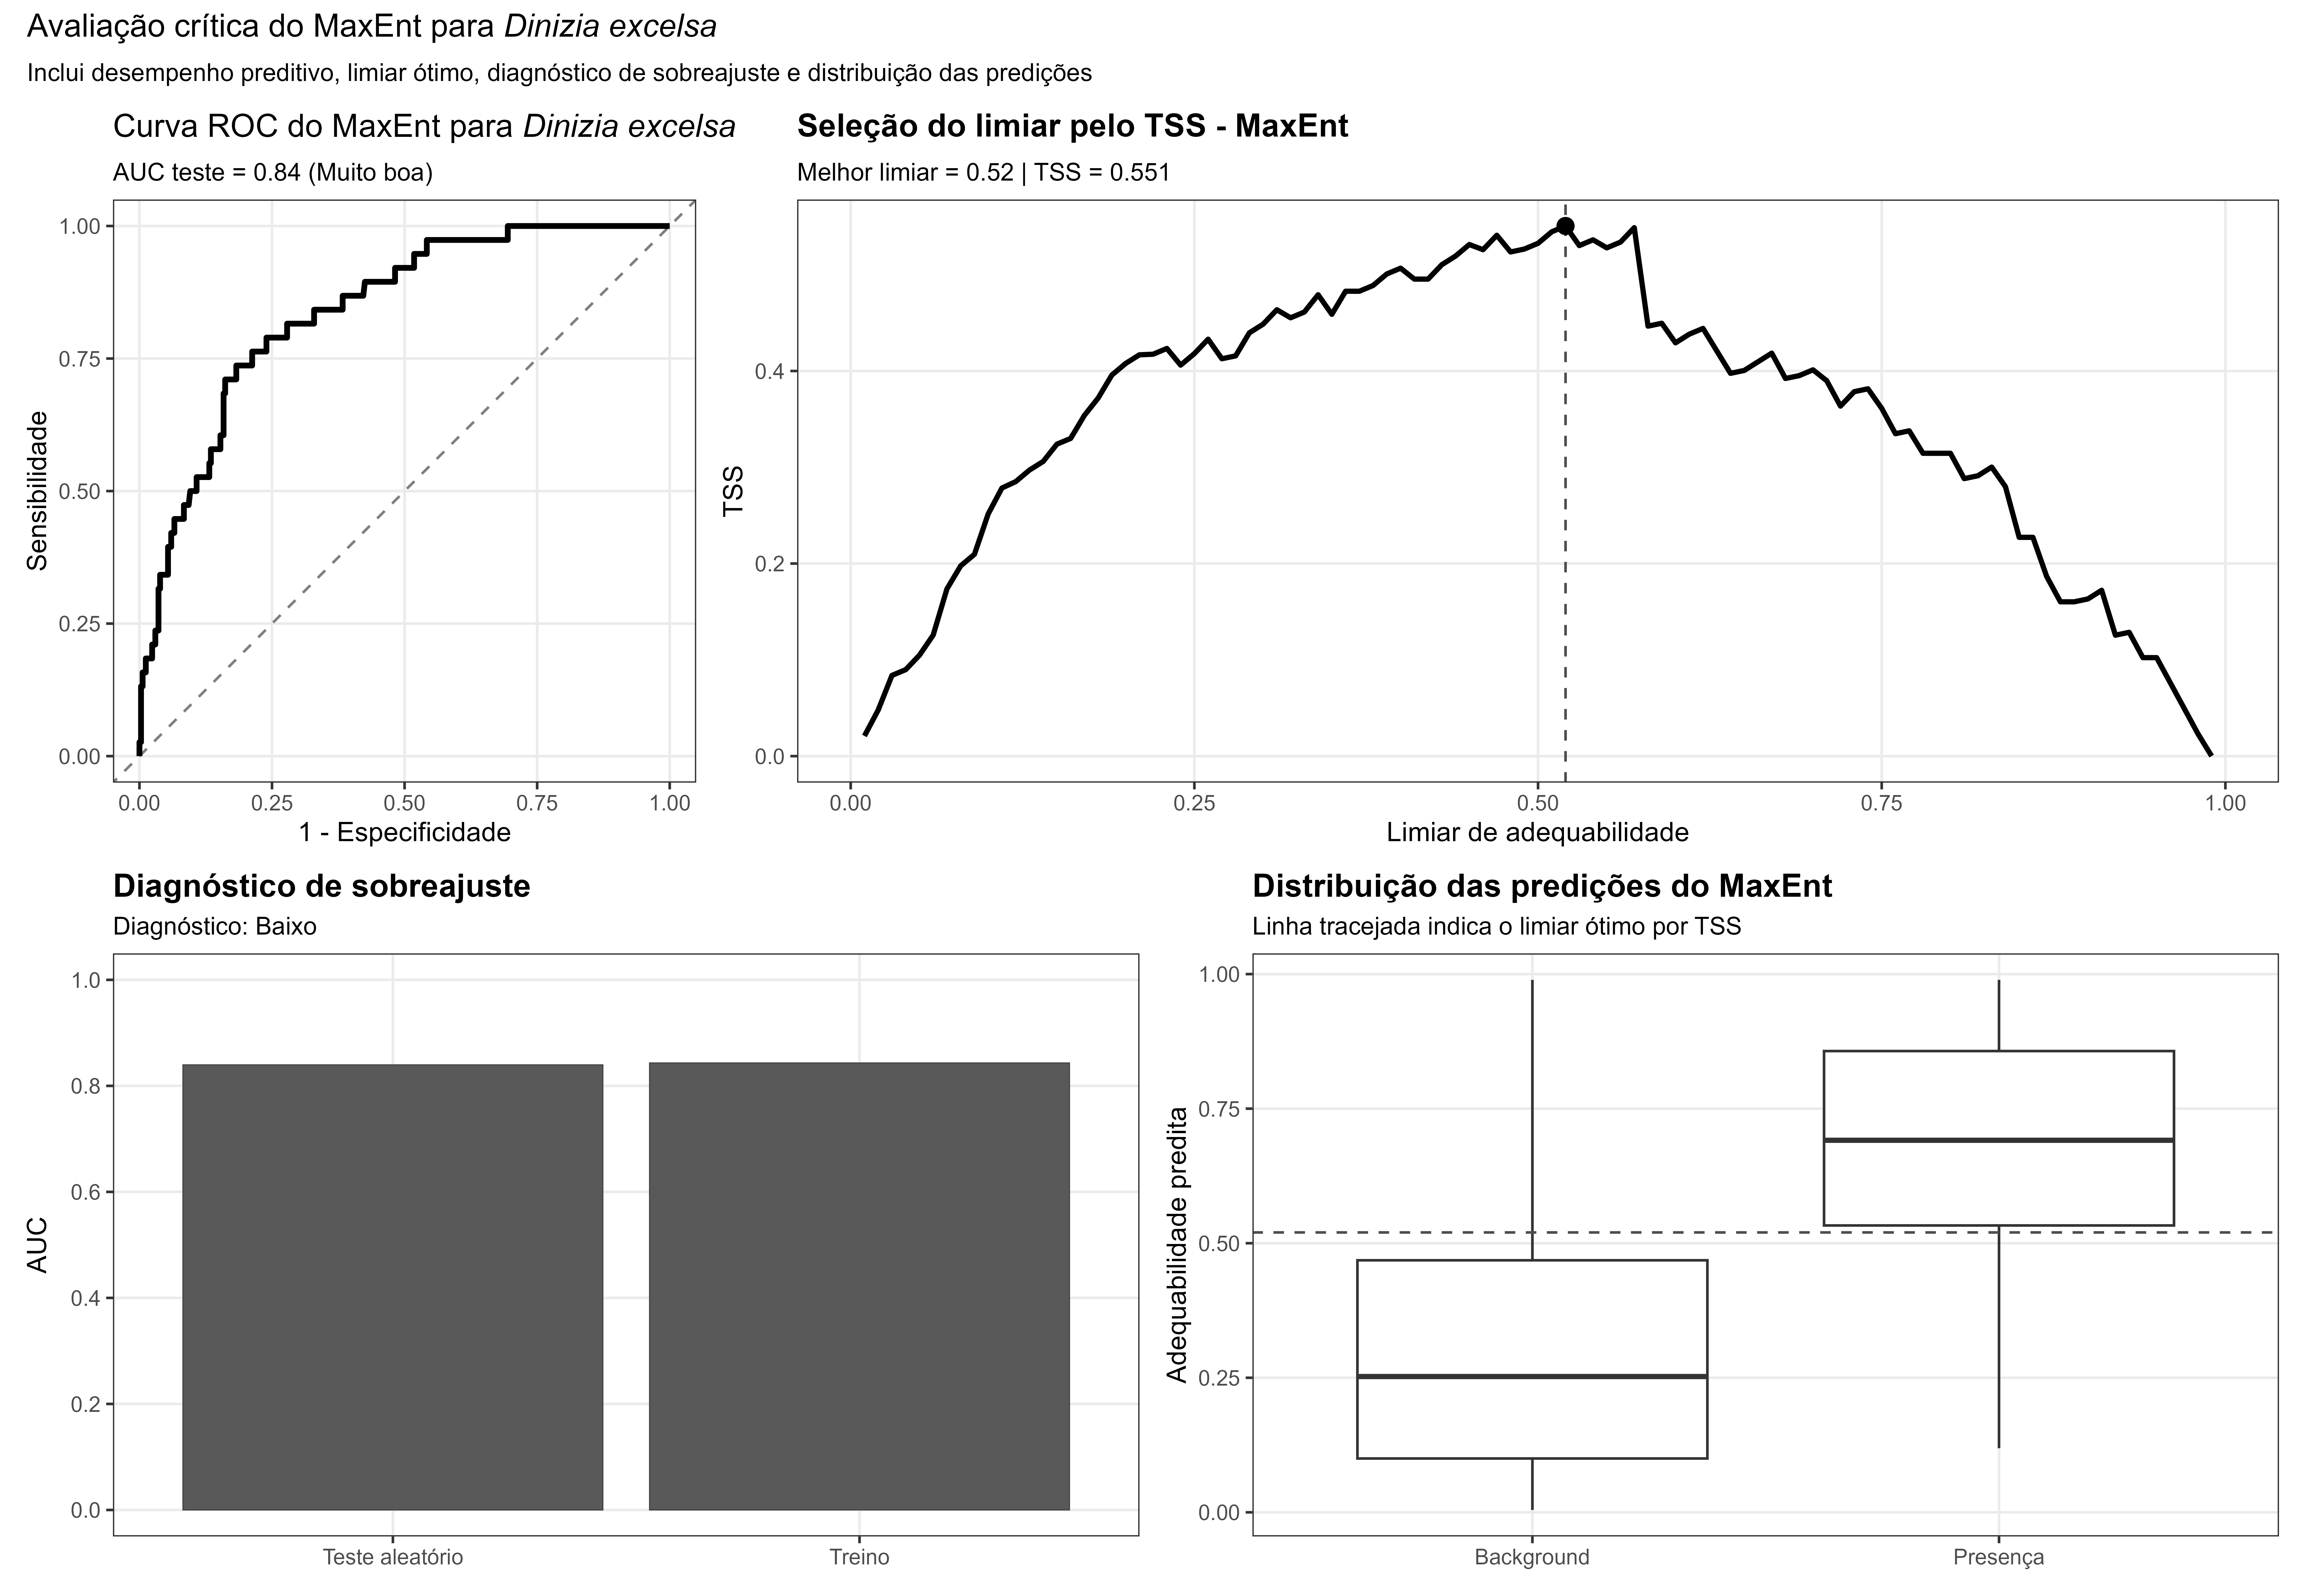
\includegraphics[width=0.78\textwidth]{figuras/unidade10/unidade10_avaliacao_maxent_patchwork.png}
  \caption{ROC curve for Maxent evaluated on the \textit{Dinizia excelsa} test set.}
  \label{fig:unidade10_roc_maxent}
\end{figure}

\section{Current Suitability Map}

The final model is projected across $M$ to produce a continuous current
suitability map.

\rscriptfile{scripts/unidade10/06_predicao_espacial_maxent.R}

\begin{figure}[H]
  \centering
  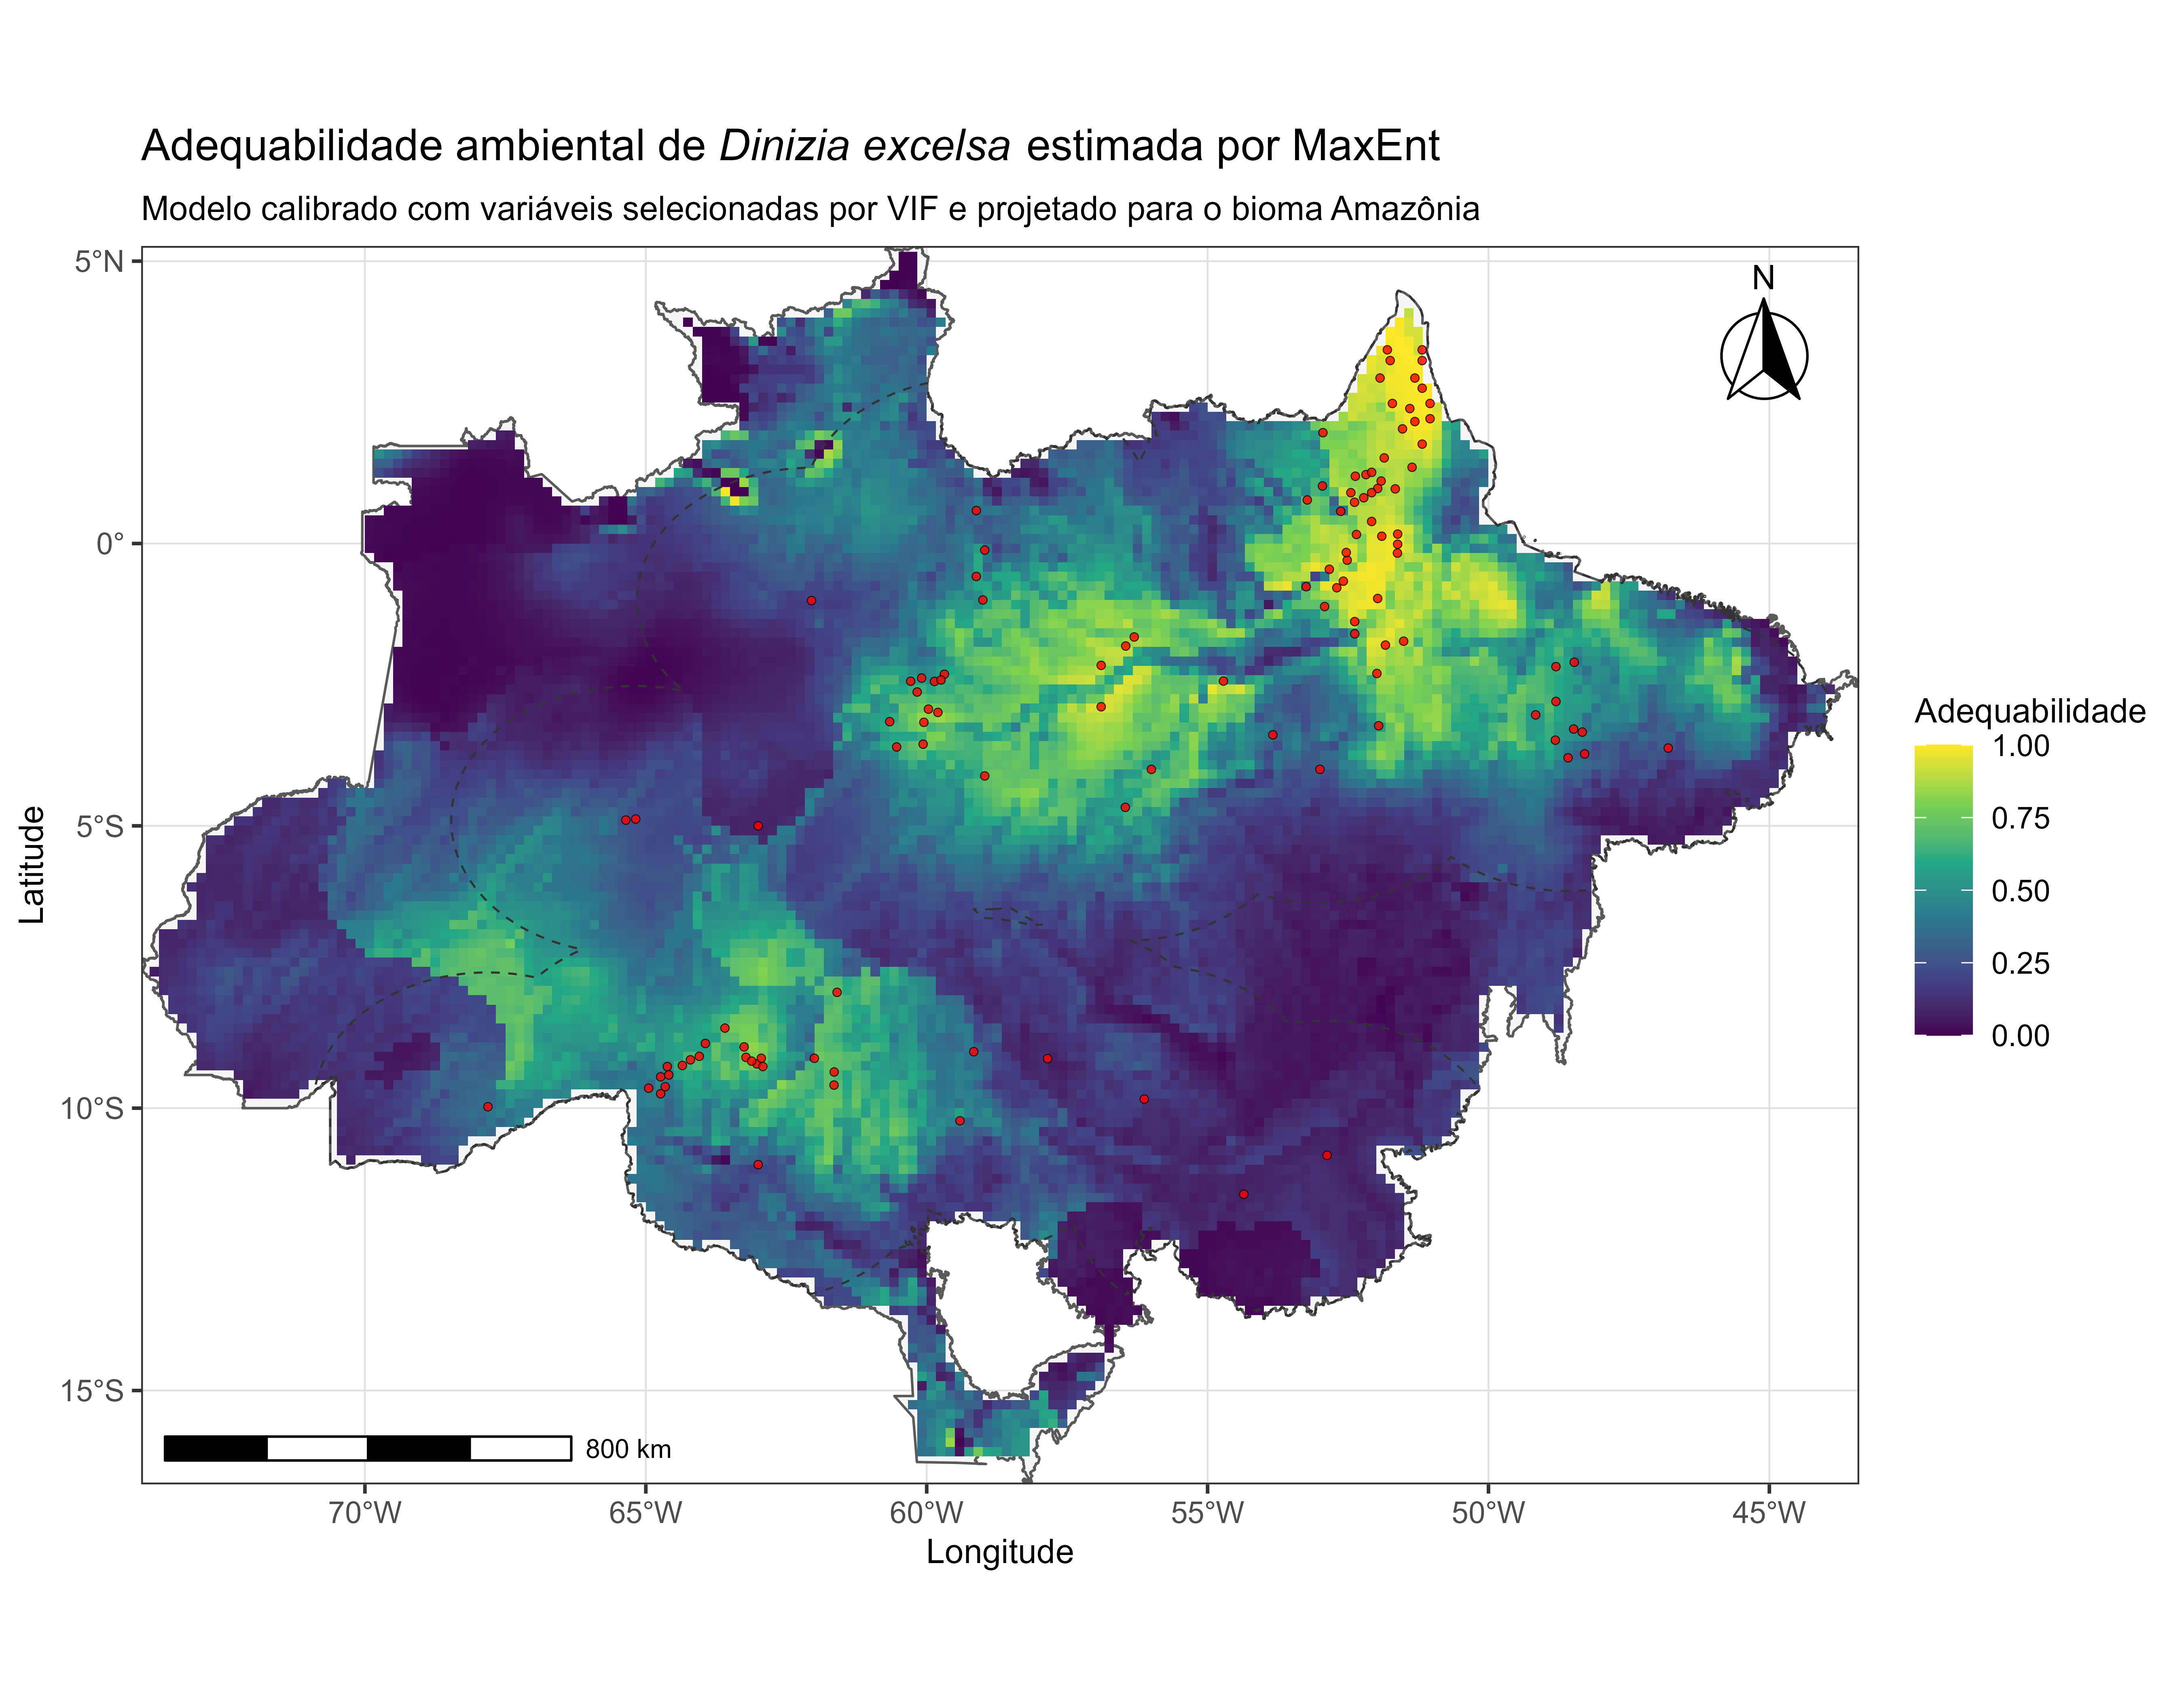
\includegraphics[width=0.88\textwidth]{figuras/unidade10/unidade10_adequabilidade_maxent.png}
  \caption{Current suitability for \textit{Dinizia excelsa} estimated by Maxent within $M$.}
  \label{fig:unidade10_adequabilidade_maxent}
\end{figure}

\section{Partial Response Curves}
\rscriptfile{scripts/unidade10/07_curvas_resposta_maxent.R}

\begin{figure}[H]
  \centering
  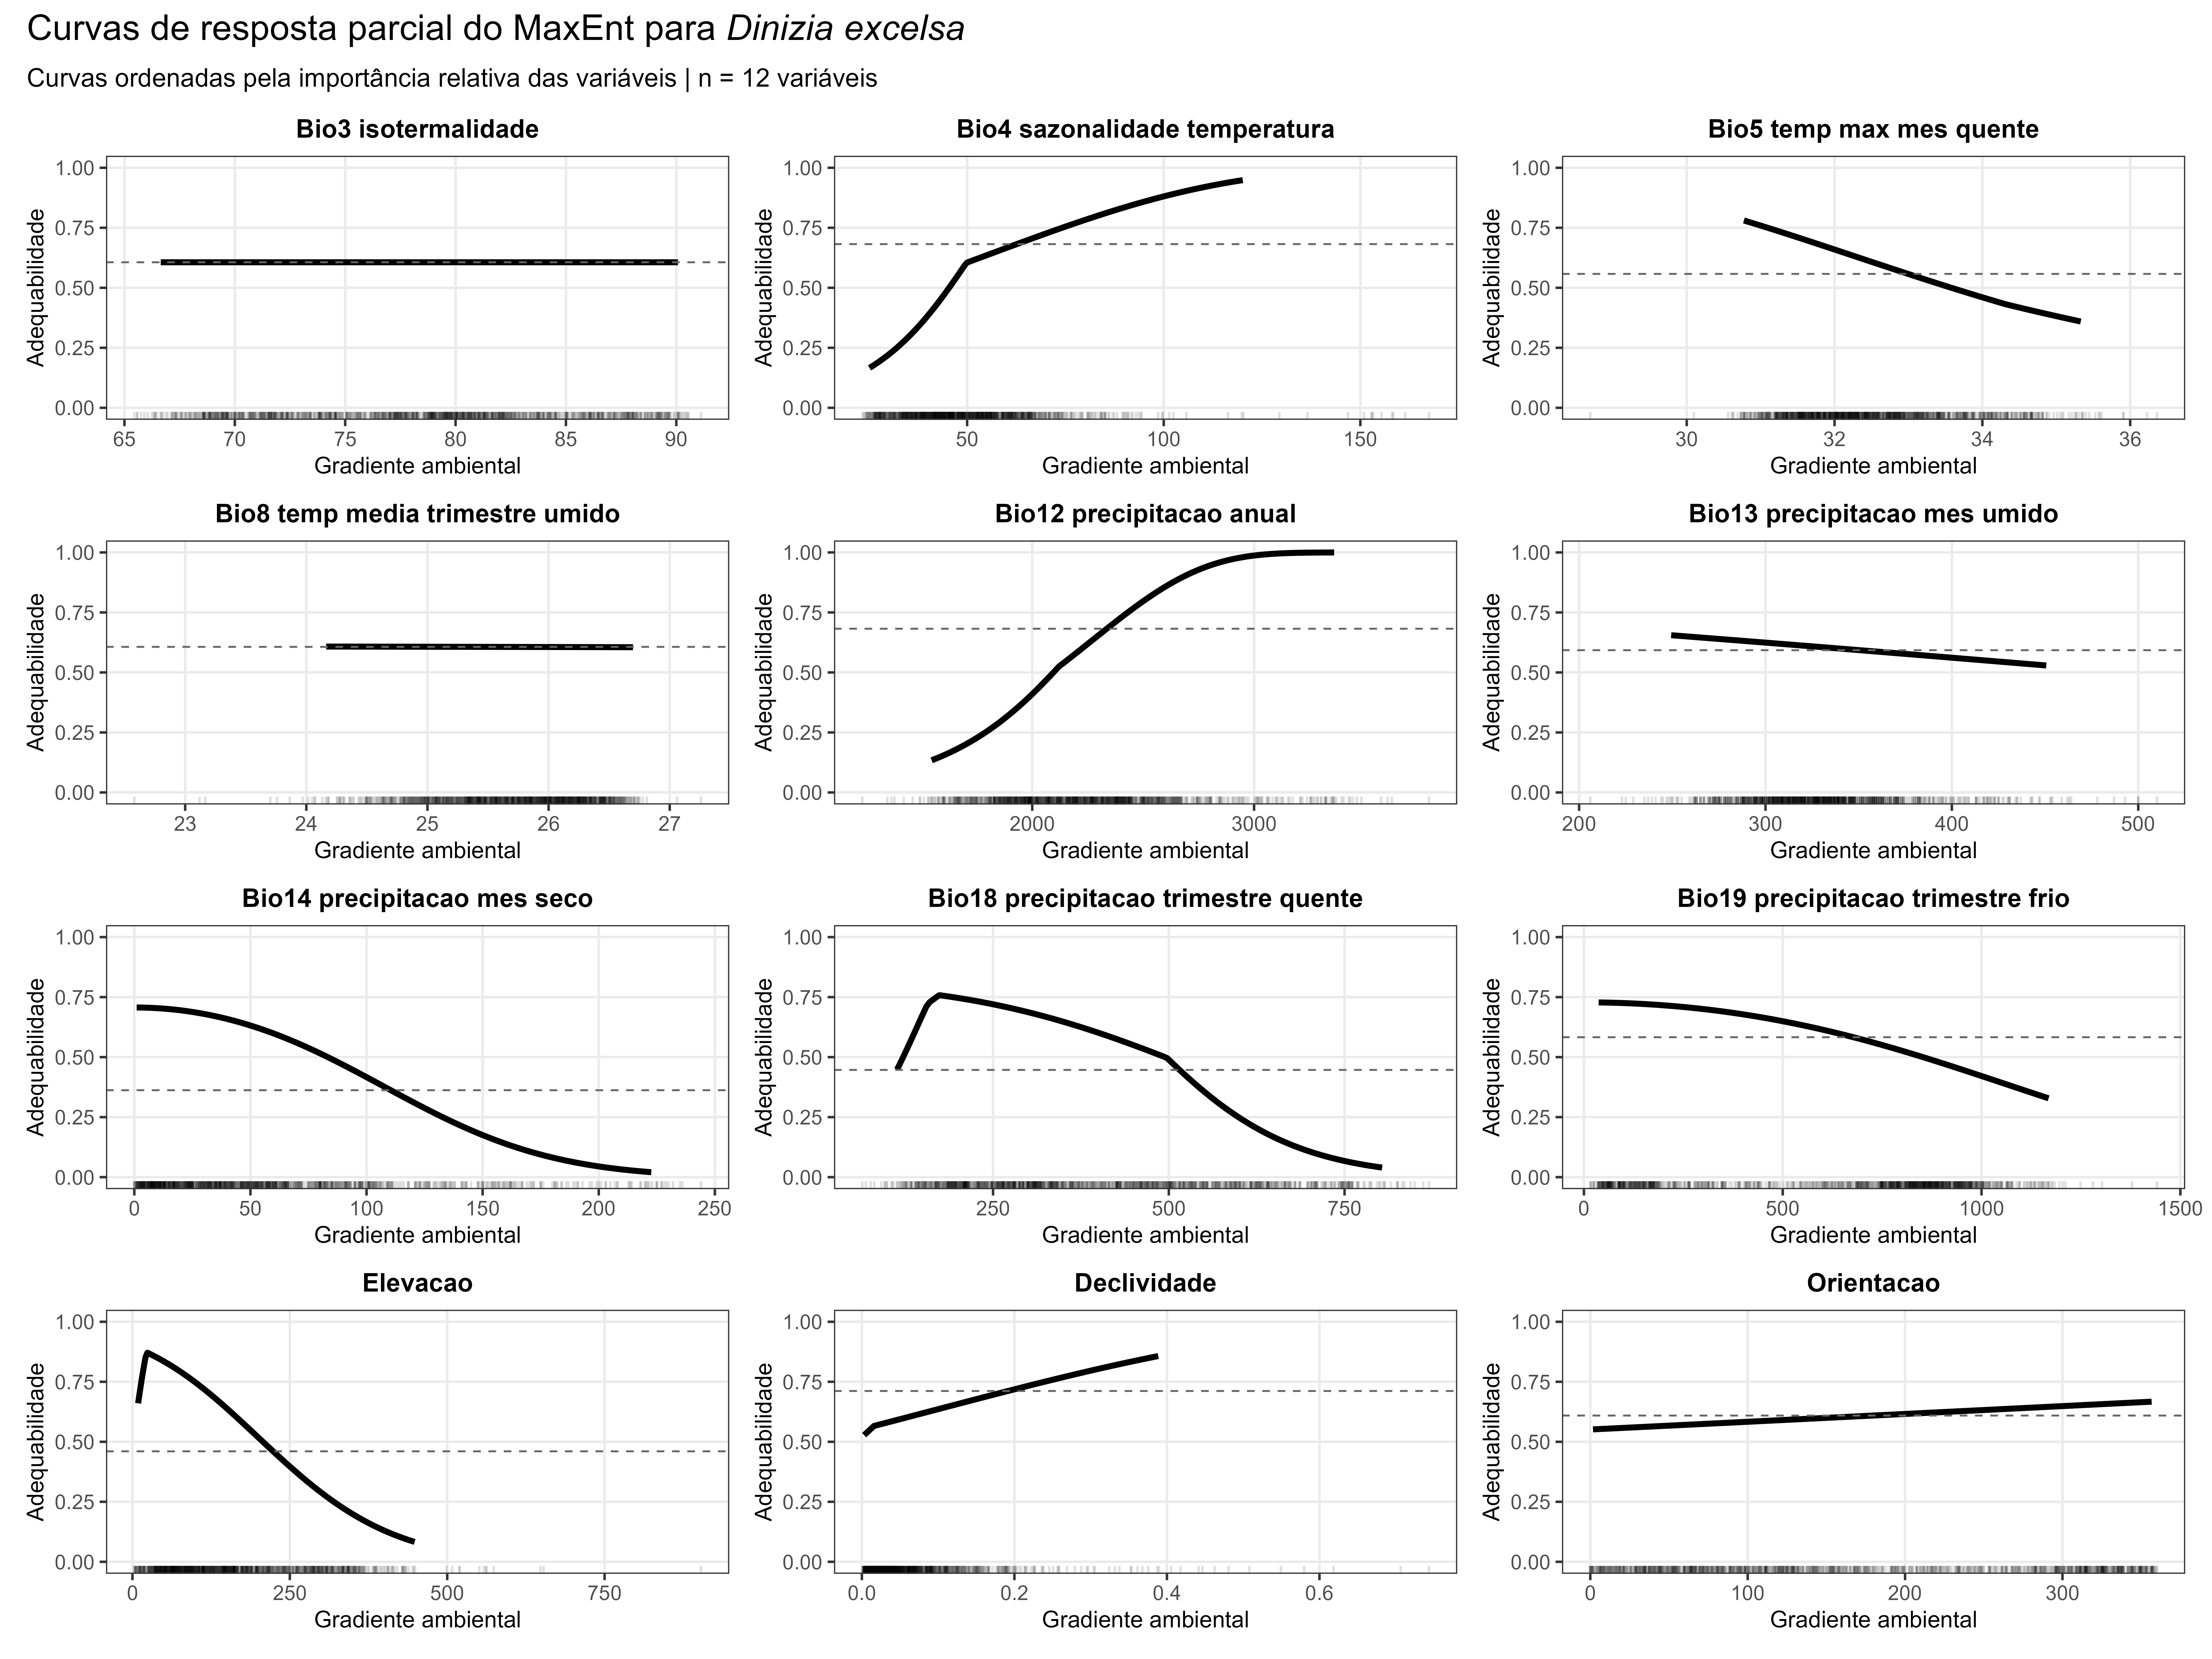
\includegraphics[width=0.96\textwidth]{figuras/unidade10/unidade10_curvas_resposta_maxent.png}
  \caption{Maxent partial response curves for the selected environmental predictors.}
  \label{fig:unidade10_curvas_resposta_maxent}
\end{figure}

\section{Comparison with Previous Models}
\rscriptfile{scripts/unidade10/08_comparar_modelos_maxent.R}

\begin{figure}[H]
  \centering
  \includegraphics[width=0.98\textwidth]{figuras/unidade10/unidade10_comparacao_modelos_maxent.png}
  \caption{Comparison of suitability maps estimated by GLM, GAM, Random Forest, BRT, and Maxent.}
  \label{fig:unidade10_comparacao_modelos}
\end{figure}

\section{Complete Pipeline}
\rscriptfile{scripts/unidade10/09_pipeline_maxent.R}

\section{Chapter Summary}

Maxent is robust and well suited to presence--background data, but responsible
application requires defensible background, feature classes, regularization,
tuning, and validation. Excessive complexity may produce detailed maps that
transfer poorly to new climates or regions.

\begin{figure}[H]
  \centering
  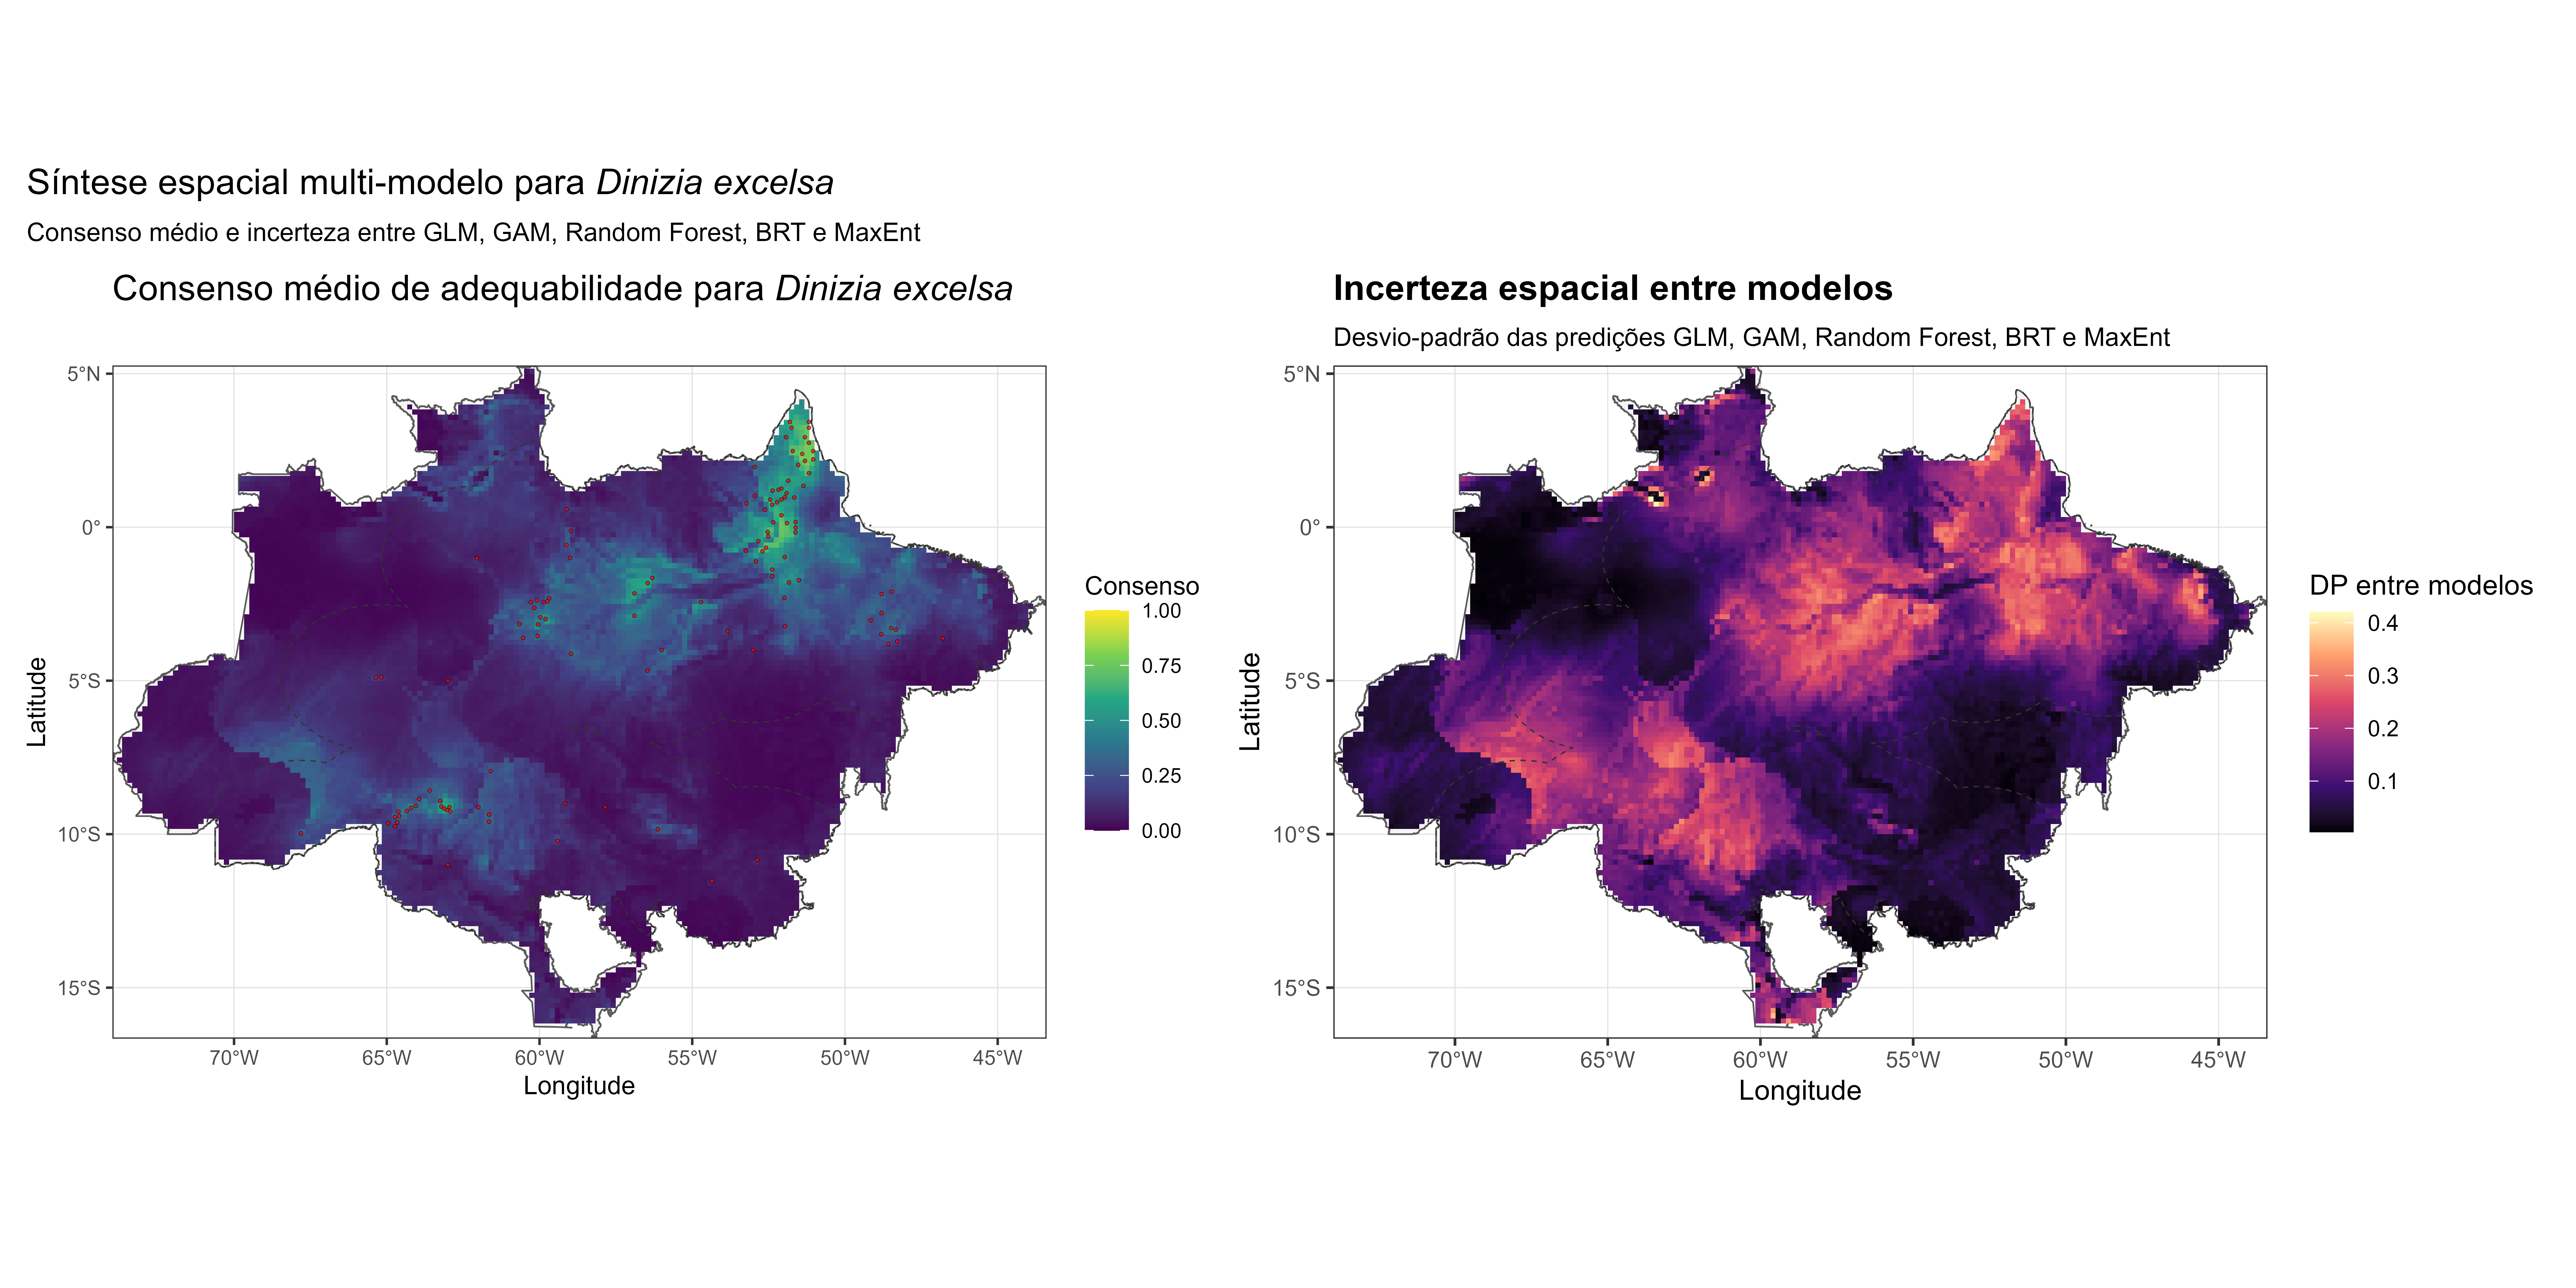
\includegraphics[width=\textwidth]{figuras/unidade10/unidade10_sintese_consenso_incerteza_glm_gam_rf_brt_maxent.png}
  \caption{Multimodel synthesis for \textit{Dinizia excelsa} across Amazonia. The left panel is mean suitability from GLM, GAM, Random Forest, BRT, and Maxent. The right panel is their standard deviation. High consensus indicates agreement on suitability; high standard deviation identifies stronger algorithmic disagreement.}
  \label{fig:unidade10_consenso_incerteza}
\end{figure}

\begin{conceito}[title={\faBook\quad Key message}]
Maxent should not be treated as a black box. Its performance depends on $M$,
background, predictor selection, regularization, and independent evaluation.
\end{conceito}

\subsection*{Comparative Synthesis of the Algorithms}

Table~\ref{tab:comparacao_algoritmos_sdm} summarizes conceptual differences,
operational strengths, methodological limitations, and interpretability.

\begin{table}[H]
\centering
\caption{Comparison of major algorithms used in species distribution modeling.}
\label{tab:comparacao_algoritmos_sdm}
\scriptsize
\setlength{\tabcolsep}{2.5pt}
\begin{tabular}{p{0.10\textwidth}p{0.14\textwidth}p{0.12\textwidth}p{0.19\textwidth}p{0.19\textwidth}p{0.14\textwidth}}
\toprule
\textbf{Method} & \textbf{Data type} & \textbf{Response} & \textbf{Strengths} & \textbf{Limitations} & \textbf{Interpretability} \\
\midrule
GLM & Presence--absence & Linear & Simple, robust, widely used & Limited flexibility for complex responses & Excellent \\
GAM & Presence--absence & Nonlinear & Flexible and interpretable & More complex than GLM & Very high \\
Random Forest & Presence--absence & Nonlinear & Strong predictive performance & Lower ecological interpretability & Moderate \\
BRT & Presence--absence & Nonlinear & Captures interactions and nonlinearities & Delicate hyperparameter tuning & Moderate \\
Maxent & Presence--background & Nonlinear & Well suited to presence-only records & Sensitive to background and sampling bias & Good \\
Ensemble & Multiple & Integrated & Represents algorithmic consensus and disagreement & More complex to interpret & Variable \\
\bottomrule
\end{tabular}
\end{table}

\subsection*{Practical Guide to Algorithm Selection}

\begin{table}[H]
\centering
\caption{Practical guide to selecting algorithms for different SDM applications.}
\label{tab:guia_escolha_algoritmos}
\small
\begin{tabular}{p{0.48\textwidth}p{0.36\textwidth}}
\toprule
\textbf{Situation} & \textbf{Candidate method} \\
\midrule
Few occurrence records & Maxent \\
Ecological interpretation of environmental effects & GLM or GAM \\
Prediction emphasizing statistical performance & Random Forest or BRT \\
Biodiversity-conservation modeling & Ensemble \\
Climate-change projections & Ensemble \\
Initial exploratory analysis & GLM \\
Ecological response curves & GAM \\
Relative predictor importance & Random Forest or BRT \\
Presence-only records & Maxent \\
Representation of algorithmic consensus and disagreement & Ensemble \\
\bottomrule
\end{tabular}
\end{table}

\begin{center}
\fbox{\begin{minipage}{0.90\textwidth}
\textbf{Methodological synthesis.} No algorithm is universally superior. Model
performance depends on data quality, $M$, predictor selection, validation, and
the ecological question. Ensembles are often useful in conservation and climate
change applications because they reduce dependence on a single algorithm and
explicitly represent between-algorithm variation; they do not automatically
eliminate bias shared by all component models.
\end{minipage}}
\end{center}

\section{Review Exercises}
\begin{enumerate}
  \item Explain the maximum entropy principle.
  \item Distinguish presence, absence, and background data.
  \item What are feature classes in Maxent?
  \item What is the role of regularization?
  \item Why can highly complex Maxent models be problematic?
  \item Why is tuning required?
  \item Compare Maxent with GLM, GAM, Random Forest, and BRT.
\end{enumerate}
